\documentclass[times, 12pt,twocolumn]{article}
\usepackage{epsf}
\usepackage{subfigure}
\usepackage{epsfig}
\usepackage{graphicX}
\newtheorem{definition}{Definition}
\newtheorem{theorem}{Theorem}
\newtheorem{proof}{Proof}
\newtheorem{problem}{Problem}
\newtheorem{algorithm}{Algorithm}
\newtheorem{protocol}{Protocol}
\newtheorem{notation}{Notation}
%\newcommand{\captionfonts}{\tiny}

%-------------------------------------------------------------------------
\begin{document}


\title{Effective Methods for Leaf Clustering Classification and Grocery Set Relations}
\author{Trevor Jacobson\\
University of Nevada, Las Vegas, USA\\
trevjacobson@gmail.com\\}



\maketitle

\thispagestyle{empty}

\begin{abstract}
Effective methods to cluster leaf image data as well as provide relationships between grocery sales data pose two interesting problems.
The leaf data allows images of leaves to be classified according to a deep set of measurements on the leaves. Each of these measurements
should allow a leaf to be classified without having to run a DNA test which can cost quite a bit of money. Therefore the motivation to
create a K-means clustering algorithm than can effectively cluster leaves could save money for researches in the field of botany.

Grocery sales data is relevant to thousands upon thousands of grocery stores around the globe. Taking a closer analysis of the sales
data generated by an anonymized store in Norway could prove useful to many grocery stores in the regions. In order to find relationships
in the set of grocery data, an efficient algorithm using the Apriori frequency item set algorithm could provide valuable insights.


\end{abstract}

\section{introduction}
We will be examining two different data sets each of which will be examined with their own algorithm. The first data set is gathered from
University of California Irvine's Machine Learning repository.\cite{Art4} The data contains key measurements on thousands of leaf samples intended to allow
classification on the leaves easily through machine learning algorithms. This research will focus on implementing a K-means clustering algorithm
in which success will be determined by using a previously known leaf and applying it to the algorithm to see if clustering is done properly.

The second data set is around 10,000 sales from an anonymized grocery store located in Norway.\cite{Art3} This data contains frequency sets for each sale,
disclosing the number of items purchased. In order to more closely examine relationships between the purchased items an Apriori algorithm will be
applied. With this algorithm we can expect to find key relationships among product purchases that will allow stores to increase sales through this
machine learning.

\section{Leaf Techniques}
Botanists all around the globe often need to examine the plant life around them when out researching in the field. In order to accurately identify plan species
DNA testing is often the go-to mechanism which can be quite expensive. In order to improve the economic situation for this field a machine learning algorithm which
can help to identify the species of plants would eliminate the need for DNA tests. This study will implement a variation of the K-means clustering algorithm that
will work with the leaf data set. For the purpose of this study success will be measured as correct classifications for a leaf. Correctness means the leaf was
accurately clustered into the species it belongs to, failure is any case where the leaf is labeled as the incorrect species.

{\bf K-means clustering algorithm}

\begin{enumerate}

\setcounter{enumi}{0}
\item Start with initial guesses for cluster centers (centroids)
\item For each data point, find closest cluster center (partitioning step)
\item Replace each centroid by average of data points in its partition
\item Iterate 1+2 until convergence

\end{enumerate}

Write $x_i = (x_{i1}, ... x_{ip})$:

If centroids are $m_1, m_2, ... m_k$, and partitions are $c_1, c_2, ... c_k$, then one can show that K-means converges to a {\it local} minimum of

\[
\sum^K_{k=1} \sum_{i\in c_k} || x_i - m_k ||^2 \ \ \ \rm Euclidean \ distance
\]

(within cluster sum of squares) \\
Utilizing this algorithm and trying to set the number of clusters to the total number of species we should see all of the same species
gather towards a cluster. The algorithm will be implemented in Java and reads from a Comma Separated Value formatted document containing the
leaf data.

\subsection{K-means Clustering Results}
Results for the K-means clustering algorithm are not promising. The best results occurred with $k=36$ where $k$ is the number of clusters provided the best results for the data set. This is likely due to the fact that there are 36 different species in the data set meaning some clusters were able to cluster to their own species which was the
goal of the algorithm. The algorithm achieved peak accuracy of 12\% for classifying the leaves to the correct species. A research paper on image classification found success when characterizing images with a word bag featuring yes or no answers to the characteristic. This approach could possibly be ported to our leaf data set to find features in the leaves that can be described as yes or no rather than the numerical data utilized.\cite{Art1} Another study found success in identifying diseased leaves through image processing using a k-means algorithm, but the data set was a single plant species likely leading to higher success compared to the 36 species analyzed in this studies leaf data set.\cite{Art2} Applying the k-means clustering algorithm has still given critical insight into the leaf data set and given time, research to a different algorithm family in machine learning may provide better results. Figures \ref{k10} and \ref{k36} located on the last page display the graphed clusters for 36 clusters and 10 clusters. The clusters are not tightly gathered which highlights the accuracy problems with the K-means clustering algorithm. Given these results, classification of leaves using K-means clustering is not the appropriate method.

\section{Grocery Techniques}
Grocers around the globe have vast amounts of transactional data that could be critical in gaining insight to increase sales. Utilizing association rule mining for transactional
databases, relationships between products should arise. These relationships will allow a grocer to group items together they may not have previously thought had relevance to one another.
Using the well known Apriori algorithm for association rule mining relationships between the Norway grocery store's items should arise. For this study we will examine rules which relate
to three or more items.

\includegraphics[scale=0.8]{apriori}

\subsection{Apriori Results}
Results from the Apriori algorithm indicate that it is a perfect fit to identify frequency relations among transactional databases. Whole milk was by far the most frequently purchased item with over 2500 of the 10000 transactions purchasing milk. The Apriori algorithm was implemented in Java to find the relationships among items, but the R langauge was used to determine confidence levels in items. The most likely purchase of three related items was whole milk, yogurt, and cereal with a confidence level of .92. If we examine relationships between five items the set changes a bit; whole milk is still included but other vegetables, rolls, water, and fruit are the most related purchases with 223 supporting transactions.
Grocery stores can make accurate predictions implementing the Apriori algorithm to their stores transactional history in order to improve sales of related groups of items as evidenced in this study. One study found that modifying the structure of a transactional database, and improving the Apriori association mining algorithm can improve results of the algorithm, a future thought to implement into this study on grocery transactions.\cite{Art5} The Apriori algorithm is key to making inferences on transactional databases as shown in this study on groceries.

\begin{figure*}

    \subfigure[10 Clusters]{
    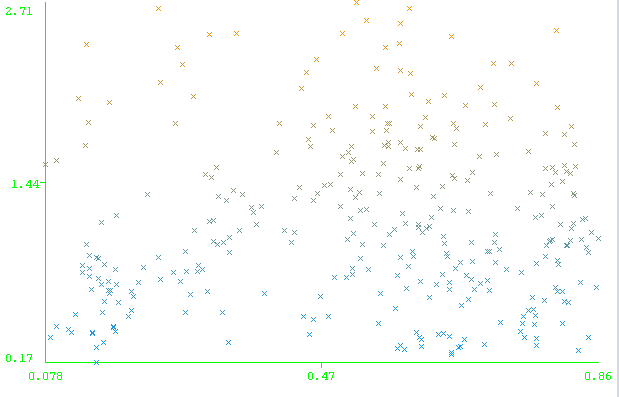
\includegraphics[scale=0.3]{kmeans10}
    \label{k10}}
    \hspace{0in}
    \subfigure[36 Clusters]{
    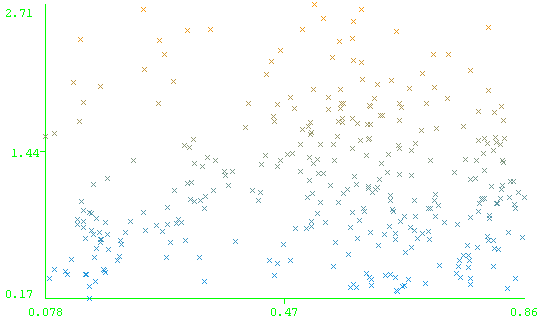
\includegraphics[scale=0.4]{kmeans36}
    \label{k36}}
\end{figure*}

\bibliographystyle{plain}
\bibliography{references01}

\end{document}
